%
% $RCSfile: domain_engineering.tex,v $
%
% Copyright (C) 2002-2008. Christian Heller.
%
% Permission is granted to copy, distribute and/or modify this document
% under the terms of the GNU Free Documentation License, Version 1.1 or
% any later version published by the Free Software Foundation; with no
% Invariant Sections, with no Front-Cover Texts and with no Back-Cover
% Texts. A copy of the license is included in the section entitled
% "GNU Free Documentation License".
%
% http://www.cybop.net
% - Cybernetics Oriented Programming -
%
% http://www.resmedicinae.org
% - Information in Medicine -
%
% Version: $Revision: 1.1 $ $Date: 2008-08-19 20:41:06 $ $Author: christian $
% Authors: Christian Heller <christian.heller@tuxtax.de>
%

\section{Domain Engineering}
\label{domain_engineering_heading}
\index{Domain Engineering}
\index{DE}
\index{Software Engineering Process}
\index{SEP}
\index{Object Oriented Analysis}
\index{OOA}
\index{Object Oriented Design}
\index{OOD}
\index{Six Pack Model}
\index{System Family Engineering}
\index{Application Engineering}
\index{AE}
\index{Analysis Phase}
\index{Design Phase}
\index{Implementation Phase}
\index{Development for Reuse}
\index{Feature Oriented Domain Analysis}
\index{FODA}
\index{Reuse driven Software Engineering Business}
\index{RSEB}
\index{Feature RSEB}
\index{FeatuRSEB}
\index{Unified Modelling Language}
\index{UML}
\index{Feature Model}

Undoubtedly, \emph{Object Oriented Programming} (OOP) (section
\ref{object_oriented_programming_heading}) is one of the most popular programming
paradigms in use today. Its application within a \emph{Software Engineering Process}
(SEP) (chapter \ref{software_engineering_process_heading}) requires two preliminary
phases called \emph{Object Oriented Analysis} (OOA) and \emph{Object Oriented Design}
(OOD).

\begin{figure}[ht]
    \begin{center}
        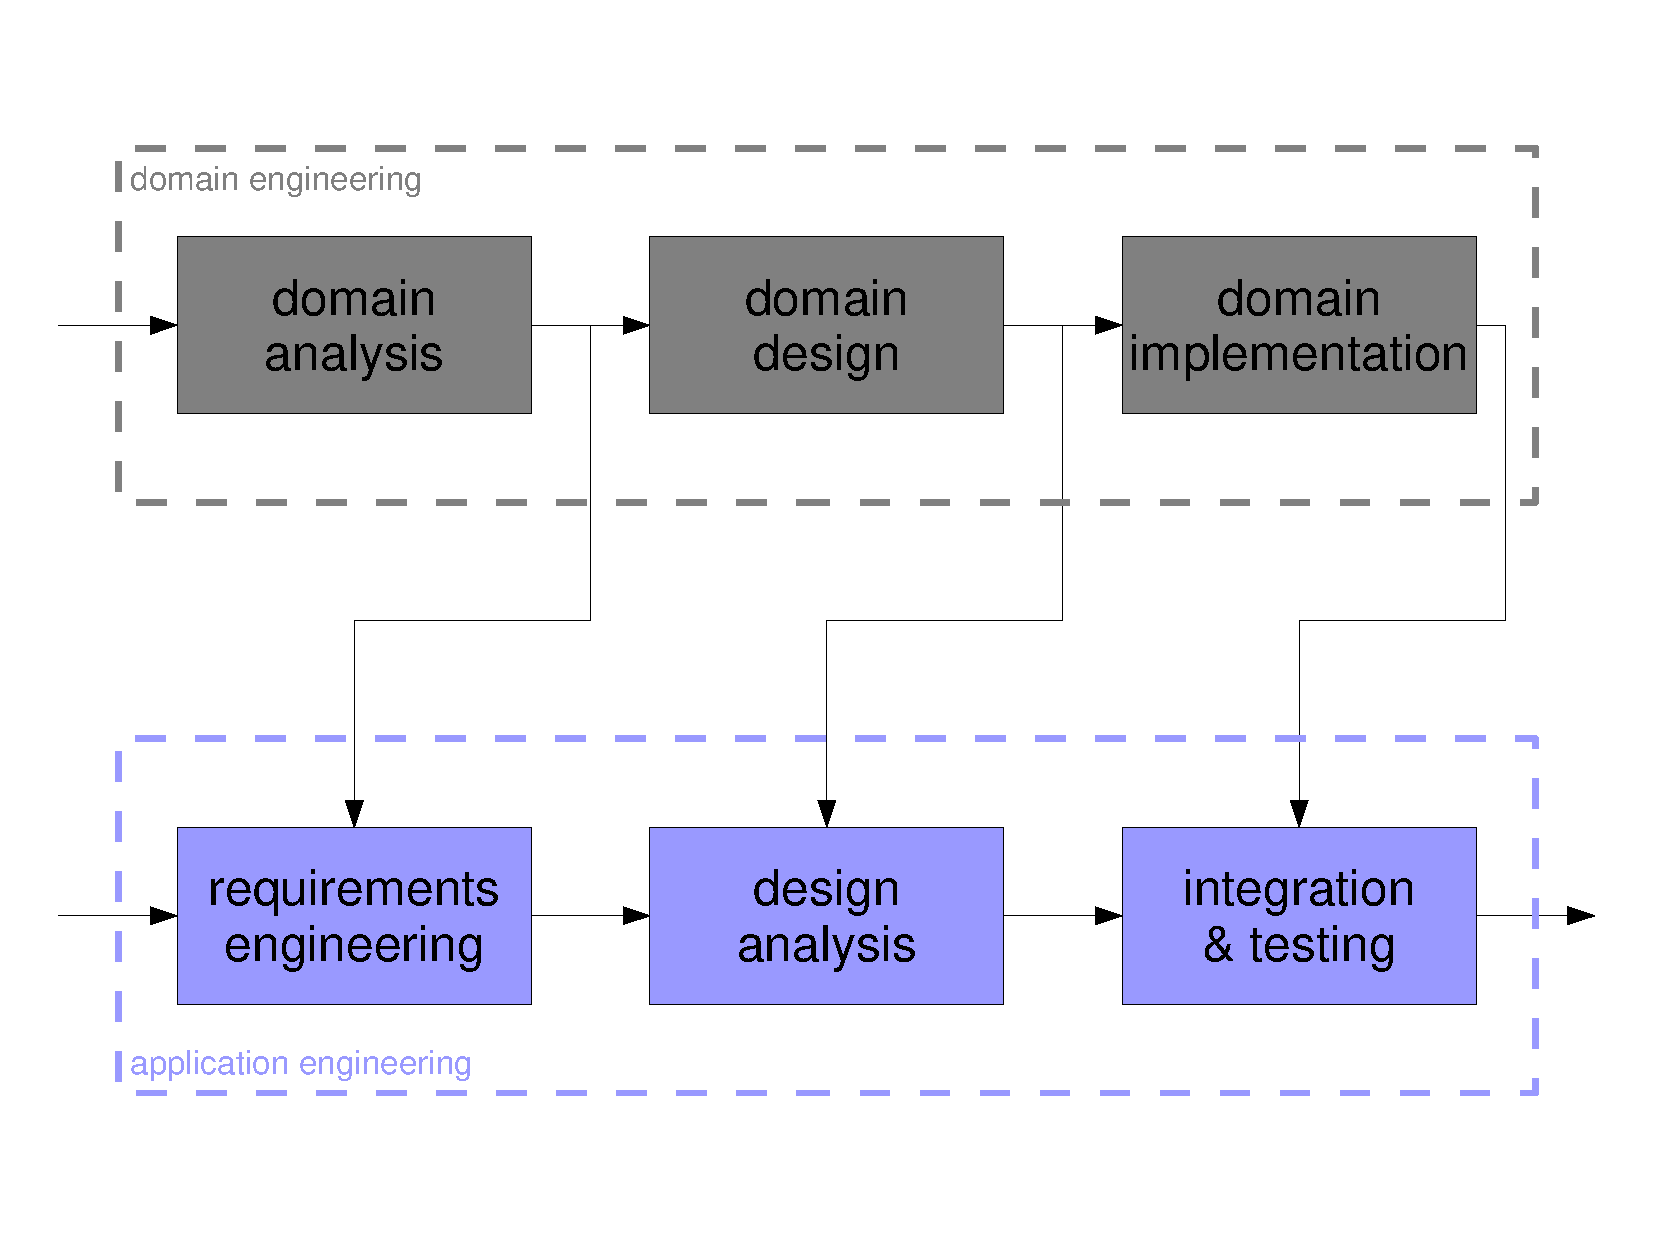
\includegraphics[scale=0.3,angle=-90]{graphic/sixpack.pdf}
        \caption{Six Pack Model of System Family Development \cite{domainengg, esaps}}
        \label{sixpack_figure}
    \end{center}
\end{figure}

The area of \emph{System Family Engineering} applies a so-called \emph{Six-Pack}
approach (figure \ref{sixpack_figure}) which is based on the separation of
\emph{Domain Engineering} (DE) and \emph{Application Engineering} (AE).
\textit{The focus of AE is a single system whereas the focus of DE is on
multiple related systems within a domain}, as \cite{domainengg} defines. Both of
them consist of analysis-, design- and implementation phases. The results of
each DE phase are \emph{fed in} as foundation for the work to be done in AE.
Most of the topics described in the previous sections
(\ref{paradigm_and_language_heading}, \ref{pattern_heading} and
\ref{component_oriented_programming_heading}) turned around techniques which
are applicable to both, DE as well as AE.

In Krzysztof Czarnecki's opinion \cite{czarnecki}, the only SEPs adequately
addressing the issue of \emph{Development for Reuse} were DE methodologies,
most of which had essentially the same structure. He writes:

\begin{quote}
    \emph{Domain Engineering} is the activity of \emph{collecting},
    \emph{organizing}, and \emph{storing} past experience in building systems or
    parts of systems in a particular domain in the form of reusable assets (i.e.
    reusable work-products), as well as providing an adequate means for
    \emph{reusing} these assets (i.e. retrieval, qualification, dissemination,
    adaptation, assembly, etc.) when building new systems.
\end{quote}

After him, the main difference between traditional OOA/ OOD- and DE methods
were that the former focus on developing \emph{Single} systems, the latter
though on developing \emph{Families} of systems. Combined with the definition
stated above (\cite{domainengg}), this means that OOA/ OOD methods may be used
for application-, but not domain engineering. Different methods and techniques
exist for DE. Many are given in \cite{wartik, arrango, fere}. Just a few of
them shall be mentioned here:

\begin{itemize}
    \item{\emph{Feature Oriented Domain Analysis} (FODA)}
    \item{\emph{Reuse driven Software Engineering Business} (RSEB)}
    \item{\emph{Feature RSEB} (FeatuRSEB)}
\end{itemize}

The RSEB methodology \cite{jacobson1997} places emphasis on purely
\emph{Object Oriented} (OO) techniques which it uses together with the
\emph{Unified Modelling Language} (UML). \emph{Features} and \emph{Feature Models}
(section \ref{feature_model_heading}), as concept, were introduced by the FODA
\cite{foda}. The combination of RSEB and FODA results in the FeatuRSEB approach
\cite{griss}. It permits a separate treatment of domain knowledge and system
functionality.

However, this work is less interested in the details of DE software development
\emph{Methods}, but rather in their \emph{Knowledge Abstraction-} and
\emph{Implementation} techniques. Some of them are investigated in the
following sections.

%
% $RCSfile: tool_and_material.tex,v $
%
% Copyright (C) 2002-2008. Christian Heller.
%
% Permission is granted to copy, distribute and/or modify this document
% under the terms of the GNU Free Documentation License, Version 1.1 or
% any later version published by the Free Software Foundation; with no
% Invariant Sections, with no Front-Cover Texts and with no Back-Cover
% Texts. A copy of the license is included in the section entitled
% "GNU Free Documentation License".
%
% http://www.cybop.net
% - Cybernetics Oriented Programming -
%
% http://www.resmedicinae.org
% - Information in Medicine -
%
% Version: $Revision: 1.1 $ $Date: 2008-08-19 20:41:09 $ $Author: christian $
% Authors: Christian Heller <christian.heller@tuxtax.de>
%

\subsection{Tool \& Material}
\label{tool_and_material_heading}
\index{Tools \& Materials Approach}
\index{Domain}
\index{Application}

In software engineering, the term \emph{Domain} stands for a special field of
business in which software systems are applied. Frequently, system development
methods distinguish between data belonging to the \emph{Domain} and
functionality defining the actual \emph{Application} working \emph{on} the
domain. The system family engineering mentioned before is one example.

This view is comparable to the well-known \emph{Tools \& Materials} approach
\cite{tandm} which is based on the distinction of \emph{active} applications
(tools) working on \emph{passive} domain data (material). \textit{Materials can
never be accessed directly, but only by using appropriate tools}, as
\cite{tandm} writes. This simple idea is an important pre-condition for the
separate treatment of \emph{System} and \emph{Knowledge}, as explained in
chapter \ref{statics_and_dynamics_heading} of this work.

%
% $RCSfile: generics.tex,v $
%
% Copyright (C) 2002-2008. Christian Heller.
%
% Permission is granted to copy, distribute and/or modify this document
% under the terms of the GNU Free Documentation License, Version 1.1 or
% any later version published by the Free Software Foundation; with no
% Invariant Sections, with no Front-Cover Texts and with no Back-Cover
% Texts. A copy of the license is included in the section entitled
% "GNU Free Documentation License".
%
% http://www.cybop.net
% - Cybernetics Oriented Programming -
%
% http://www.resmedicinae.org
% - Information in Medicine -
%
% Version: $Revision: 1.1 $ $Date: 2008-08-19 20:41:06 $ $Author: christian $
% Authors: Christian Heller <christian.heller@tuxtax.de>
%

\subsection{Generics}
\label{generics_heading}
\index{Generics}
\index{Generic Programming}
\index{Function Template}
\index{Class Template}
\index{Standard Template Library}
\index{STL}
\index{Eiffel}
\index{Java}
\index{VB.NET}
\index{C\#}
\index{Reuse through Parameterisation}
\index{Dynamic Typing}

\emph{Generic Programming} received its name from the \emph{Generics} it uses.
Wikipedia \cite{wikipedia} writes: \textit{Generics is a technique that allows
one value to take different datatypes (so-called polymorphism) as long as
certain contracts such as subtypes and signature are kept.} \emph{Templates}
are one technique providing generics. They allow the writing of code without
considering the data type that code will eventually be used with. Two kinds of
templates exist \cite{wikipedia}:

\begin{itemize}
    \item[-] \emph{Function Template:} behaving like a function that can accept
        arguments of many different types
    \item[-] \emph{Class Template:} extending the same concept to classes;
        often used to make generic containers
\end{itemize}

Using templates of the C++ \emph{Standard Template Library} (STL) \cite{stl},
a list may be declared by writing \texttt{list<T>}, where \emph{T} represents
the type that may be substituted as needed. A linked list of integers, for
example, would be created with \texttt{list<int>}. After \cite{wikipedia},
there are three primary drawbacks to the use of templates:

\begin{enumerate}
    \item Less portable code due to the poor support for templates in compilers
    \item Difficult development of templates due to unhelpful error messages
        produced by compilers
    \item Bloated code due to the extra code (instantiated template) generated
        by compilers
\end{enumerate}

Meanwhile, many other OOP languages like \emph{Eiffel}, \emph{Java},
\emph{VB.NET} and \emph{C\#} provide generic facilities. Being used to improve
the customisability of code at compile time, they retain the efficiency of
statically configured code. However, in practice (own experience of the author)
it is often hard for programmers to understand and handle generic techniques.
Czarnecki \cite{czarnecki}, who summarises generic programming as \textit{Reuse
through Parameterisation}, criticises that it: \textit{limits code generation
to substituting generic type parameters with concrete types and welding together
pre-existing fragments of code in a fixed pattern.} \emph{Dynamic Typing}
(section \ref{typeless_programming_heading}) is one possibility to circumvent
the need for generic programming. The interpreter program introduced in chapter
\ref{cybernetics_oriented_interpreter_heading} uses dynamic typing; it
references all knowledge via neutral pointers whose meaning gets determined
only at runtime.

%
% $RCSfile: domain_specific_language.tex,v $
%
% Copyright (C) 2002-2008. Christian Heller.
%
% Permission is granted to copy, distribute and/or modify this document
% under the terms of the GNU Free Documentation License, Version 1.1 or
% any later version published by the Free Software Foundation; with no
% Invariant Sections, with no Front-Cover Texts and with no Back-Cover
% Texts. A copy of the license is included in the section entitled
% "GNU Free Documentation License".
%
% http://www.cybop.net
% - Cybernetics Oriented Programming -
%
% http://www.resmedicinae.org
% - Information in Medicine -
%
% Version: $Revision: 1.1 $ $Date: 2008-08-19 20:41:06 $ $Author: christian $
% Authors: Christian Heller <christian.heller@tuxtax.de>
%

\subsection{Domain Specific Language}
\label{domain_specific_language_heading}
\index{Domain Specific Language}
\index{DSL}
\index{General Purpose Language}
\index{GPL}
\index{Little Language}
\index{Application Language}
\index{Macro}
\index{Very High Level Language}
\index{GraphViz DOT}
\index{Mathematica}
\index{Yet Another Compiler Compiler}
\index{YACC}
\index{Universal Interactive Executive}
\index{UNIX}
\index{UNIX Shell Script}
\index{Lisp}
\index{Smalltalk}
\index{In-Language DSL}
\index{C++}
\index{Ruby}

While a \emph{General Purpose Language} (GPL), no matter if in form of a
scripting- or compiled programming language, can be used for performing a
variety of different tasks, a (usually declarative) \emph{Domain Specific Language}
(DSL), though less comprehensive, is more expressive in a special domain
context \cite{deursen}. After \cite{wikipedia}, DSLs may: \textit{enhance the
productivity, reliability, maintainability, portability and reusability of
software.} In Czarnecki's words \cite{czarnecki}, DSLs: \textit{increase the
abstraction level for a particular problem domain} and, being highly
intentional: \textit{allow users to work closely with domain concepts.}

Several synonyms are used to label a DSL, for example: \emph{Little Language},
\emph{Application Language}, \emph{Macro} or \emph{Very High Level Language}
\cite{wikipedia}. To the numerous representatives belong simple spreadsheet
\emph{Macros} as well as graph definition languages like \emph{GraphViz}'s
\emph{DOT} \cite{graphviz}, languages for numerical and symbolic computation as
used in \emph{Mathematica} \cite{mathematica}, or parser generator languages
like \emph{Yet Another Compiler Compiler} (YACC), found on
\emph{Universal Interactive Executive} (UNIX) systems. Even UNIX
\emph{Shell Scripts} can be considered a DSL, with emphasis on data
organisation. Further DSLs exist, yet are the boundaries between the concepts
of domain specific- and other languages quite blurry \cite{wikipedia}.

Martin Fowler \cite{fowlerdsl} mentions that the \emph{Lisp} \cite{commonlisp}
and \emph{Smalltalk} \cite{smalltalk} communities, rather than defining a new
language, frequently morph the GPL into a DSL, in a \emph{bottom-up} manner.
Such \emph{In-Language} DSLs, as he calls them, use constructs of the
programming language itself. Wondering why, programming in Smalltalk, he never
really felt the need to use a separate language, while, programming in C++/
Java/ C\#, quite often he did, he concludes \cite{fowlerdsl} that: \textit{the
more suitable languages (are) minimalist ones with a single basic idea that's
deeper and simpler than traditional languages (function application for lisp,
objects and messages for smalltalk)}, and finds that it is the
\textit{friendliness towards in-language DSLs} rather than \textit{static
versus dynamic typing} that let many software developers \textit{enjoy
programming in Smalltalk or Ruby so much more than in Java or C\#}.

Besides their limited usability outside the special domain they were created
for, to the problems that the usage of DSLs brings with belong after
\cite{menzies}:

\begin{itemize}
    \item[-] High cost of designing, implementing, and maintaining a DSL
    \item[-] Difficult finding of the proper scope
    \item[-] Difficult balancing between domain-specificity and GPL constructs
    \item[-] Potential loss of efficiency when compared with hand-coded software
\end{itemize}

The language introduced in chapter \ref{cybernetics_oriented_language_heading}
is simple and just because of that flexible enough to be applicable for
modelling the knowledge of arbitrary domains. It might have the potential to
replace some of the existing DSLs, the investigation of what is out of the
scope of this work, though.

%
% $RCSfile: specification_language.tex,v $
%
% Copyright (C) 2002-2008. Christian Heller.
%
% Permission is granted to copy, distribute and/or modify this document
% under the terms of the GNU Free Documentation License, Version 1.1 or
% any later version published by the Free Software Foundation; with no
% Invariant Sections, with no Front-Cover Texts and with no Back-Cover
% Texts. A copy of the license is included in the section entitled
% "GNU Free Documentation License".
%
% http://www.cybop.net
% - Cybernetics Oriented Programming -
%
% http://www.resmedicinae.org
% - Information in Medicine -
%
% Version: $Revision: 1.1 $ $Date: 2008-08-19 20:41:09 $ $Author: christian $
% Authors: Christian Heller <christian.heller@tuxtax.de>
%

\subsection{Specification Language}
\label{specification_language_heading}
\index{Specification Language}
\index{Unified Modeling Language}
\index{UML}
\index{Feature Model}
\index{Z Specification Language}
\index{B Specification Language}
\index{Vienna Development Method - Specification Language}
\index{VDM-SL}
\index{Specification and Description Language}
\index{SDL}
\index{Extended Meta Language}
\index{Extended ML}

A \emph{Specification Language}, after \cite{wikipedia}, were a formal language
used during system analysis and design, as opposed to a \emph{Programming Language},
which were a mostly directly executable formal language used to implement a system.
As its name already indicates, a specification language describes systems at a much
higher abstract level than a programming language does. But that also means that it:
\textit{must be subject to a process of refinement (the filling-in of implementation
detail), before it can actually be implemented}, as \cite{wikipedia} writes.

Many kinds of specification languages exist. Being a de facto standard, only
the first two of those representatives listed following are introduced in
slightly more detail below:

\begin{itemize}
    \item[-] \emph{Unified Modeling Language} (UML) \cite{uml}
    \item[-] \emph{Feature Model} \cite{foda}
    \item[-] \emph{Z Specification Language} \cite{zspeclang} and
        \emph{B Specification Language} \cite{zb2005}
    \item[-] \emph{Vienna Development Method - Specification Language} (VDM-SL) \cite{vdmsl}
    \item[-] \emph{Specification and Description Language} (SDL) \cite{sdl}
    \item[-] \emph{Extended Meta Language} (Extended ML) \cite{extendedml}
\end{itemize}

%
% $RCSfile: unified_modeling_language.tex,v $
%
% Copyright (C) 2002-2008. Christian Heller.
%
% Permission is granted to copy, distribute and/or modify this document
% under the terms of the GNU Free Documentation License, Version 1.1 or
% any later version published by the Free Software Foundation; with no
% Invariant Sections, with no Front-Cover Texts and with no Back-Cover
% Texts. A copy of the license is included in the section entitled
% "GNU Free Documentation License".
%
% http://www.cybop.net
% - Cybernetics Oriented Programming -
%
% http://www.resmedicinae.org
% - Information in Medicine -
%
% Version: $Revision: 1.1 $ $Date: 2008-08-19 20:41:09 $ $Author: christian $
% Authors: Christian Heller <christian.heller@tuxtax.de>
%

\subsubsection{Unified Modeling Language}
\label{unified_modeling_language_heading}
\index{Unified Modeling Language}
\index{UML}
\index{Class Diagram}
\index{Activity Diagram}
\index{Sequence Diagram}
\index{Use Case Diagram}
\index{State Machine Diagram}
\index{State Chart Diagram}
\index{Component Diagram}
\index{Deployment Diagram}
\index{Object Diagram}
\index{Instance Diagram}
\index{Package Diagram}
\index{Communication Diagram}
\index{Collaboration Diagram}
\index{Composite Structure Diagram}
\index{Interaction Overview Diagram}
\index{Timing Diagram}
\index{UML Diagram Type}
\index{Object Constraint Language}
\index{OCL}
\index{Structure Diagram}
\index{Behaviour Diagram}
\index{Interaction Diagram}
\index{Functional Model}
\index{Object Model}
\index{Dynamic Model}
\index{UML Tool}
\index{Computer Aided Software Engineering Tool}
\index{CASE Tool}
\index{Object Process Diagram}
\index{OPD}
\index{Entity Relationship Diagram}
\index{ERD}

Meanwhile, the probably most famous modelling- and specification language is
the \emph{Unified Modeling Language} (UML) \cite{uml, booch}. It uses a
graphical notation defining a number of diagrams. UML 2.x specifications
\cite{uml} extend the number of different diagram types from 9 (UML 1.x) to 13.
A good overview is given by Ambler in \cite{ambler2005}, which table
\ref{diagrams_table} reproduces in adapted form, showing only \emph{some}
diagram elements. The column \emph{Importance} contains a certainly subjective
recommendation of Ambler, indicating the \emph{Learning Priority} the single
diagram types have in his opinion (which the author of this work supports).

\begin{table}[ht]
    \begin{center}
        \begin{footnotesize}
        \begin{tabular}{| p{35mm} | p{55mm} | p{15mm} |}
            \hline
            \textbf{Diagram} & \textbf{Elements} & \textbf{Importance}\\
            \hline
            Class (CsD) & Class, Inheritance, Association & High\\
            \hline
            Activity (AD) & Activity, Flow, Fork/ Join, Condition, Decision/ Merge & High\\
            \hline
            Sequence (SD) & Object, Lifeline, Activation Box (Method-Invocation Box), Message & High\\
            \hline
            Use Case (UCD) & Use Case, Actor, Association & Medium\\
            \hline
            State Machine (SMD), formerly State Chart Diagram & State, Transition & Medium\\
            \hline
            Component (CmD) & Component, Interface, Dependency & Medium\\
            \hline
            Deployment (DD) & Node, Connection & Medium\\
            \hline
            Object (ObD), also referred to as Instance Diagram & Object, Relationship & Low\\
            \hline
            Package (PD) & Package, Dependency & Low\\
            \hline
            Communication (CoD), formerly Collaboration Diagram & Object, Association & Low\\
            \hline
            Composite Structure (CSD) & Collaboration, Object, Role & Low\\
            \hline
            Interaction Overview (IOD) & Interaction Frame, Interaction Occurrence Frame & Low\\
            \hline
            Timing (TiD) & Object, Lifeline, State, Timing Constraint & Low\\
            \hline
        \end{tabular}
        \end{footnotesize}
        \caption{UML 2.x Diagram Types \cite{ambler2005}}
        \label{diagrams_table}
    \end{center}
\end{table}

One extension to the UML that is now also part of the corresponding de-facto
standard, is the \emph{Object Constraint Language} (OCL). Being a declarative
language, it describes rules applying to UML models, in a precise text format.
This is because not all rules can be expressed by diagrammatic notation
\cite{wikipedia}. The range of possible rules comprises constraints like pre-
and post-conditions or object query expressions. \cite{ocl}

A common classification distinguishes UML diagrams as follows \cite{ambler2005}:

\begin{enumerate}
    \item \emph{Structure:} CsD, CmD, CSD, DD, ObD, PD
    \item \emph{Behaviour:} AD, SMD, UCD
    \item \emph{Interaction:} CoD, IOD, SD, TiD
\end{enumerate}

Others share the information represented by the diagrams according to an
underlying, independently existing model \cite{wikipedia}:

\begin{itemize}
    \item[-] \emph{Functional Model} (UCD): Functionality of the system from
        the user's point of view
    \item[-] \emph{Object Model} (CsD): Structure and substructure of the
        system using objects, attributes, operations, and associations
    \item[-] \emph{Dynamic Model} (AD, SD, SCD): Internal behaviour of the
        system
\end{itemize}

A program working with UML diagrams is called \emph{UML Tool}, or more exactly
\emph{Computer Aided Software Engineering} (CASE) tool. Many of these programs
have developed and matured, over the past decade of years. Besides the standard
UML diagram types, they offer source code parsing and -generation,
documentation creation and more. Some tools introduced their own extensions to
the UML de-facto standard, for example: \emph{Object Process Diagram} (OPD)
\cite{burkhardt} and \emph{Entity Relationship Diagram} (ERD) \cite{otw}. The
description of a hypothetic design tool suggested for the language being
introduced in chapter \ref{cybernetics_oriented_language_heading} will refer
back to the UML diagrams as mentioned in this section, and suggest a different
way to categorise them. Further, chapter \ref{cybernetics_oriented_language_heading}
will try to define four diagram types to be used in conjunction with the
language described in it.

%
% $RCSfile: feature_model.tex,v $
%
% Copyright (C) 2002-2008. Christian Heller.
%
% Permission is granted to copy, distribute and/or modify this document
% under the terms of the GNU Free Documentation License, Version 1.1 or
% any later version published by the Free Software Foundation; with no
% Invariant Sections, with no Front-Cover Texts and with no Back-Cover
% Texts. A copy of the license is included in the section entitled
% "GNU Free Documentation License".
%
% http://www.cybop.net
% - Cybernetics Oriented Programming -
%
% http://www.resmedicinae.org
% - Information in Medicine -
%
% Version: $Revision: 1.1 $ $Date: 2008-08-19 20:41:06 $ $Author: christian $
% Authors: Christian Heller <christian.heller@tuxtax.de>
%

\subsubsection{Feature Model}
\label{feature_model_heading}
\index{Feature Model}
\index{Feature Modelling}
\index{System Family}
\index{Software Product Line}
\index{Feature Driven Design}
\index{Software Engineering Process}
\index{SEP}
\index{Feature Oriented Domain Analysis}
\index{FODA}
\index{Traceability}

Czarnecki \cite{czarnecki} sees \emph{Feature Modelling}, a technique for
analysing and capturing \emph{common} and \emph{variable} features of a family
of systems as well as their inter-dependencies in form of a \emph{Feature Model},
as the main contribution of domain engineering to OOA/ OOD methods. The
\emph{System Families}, also called \emph{Software Product Lines}, whose
development feature models shall support, are described by Kai Boellert
\cite{boellert} as \textit{group of software systems that are developed from a
common set of reusable components}. Czarnecki writes:

\begin{quote}
    \emph{Feature Models} represent the configurability aspect of reusable
    software at an abstract level, i.e. without committing to any particular
    implementation technique such as inheritance, aggregation, or parameterized
    classes. Developers construct the initial models of the reusable software
    in the form of feature models and use them to \emph{guide} the design and
    implementation (also called \emph{Feature-driven Design}). To a reuser, on
    the other hand, feature models represent an \emph{overview} of the
    functionality of the reusable software and a guide to \emph{configuring} it
    for a specific usage context.
\end{quote}

\begin{figure}[ht]
    \begin{center}
        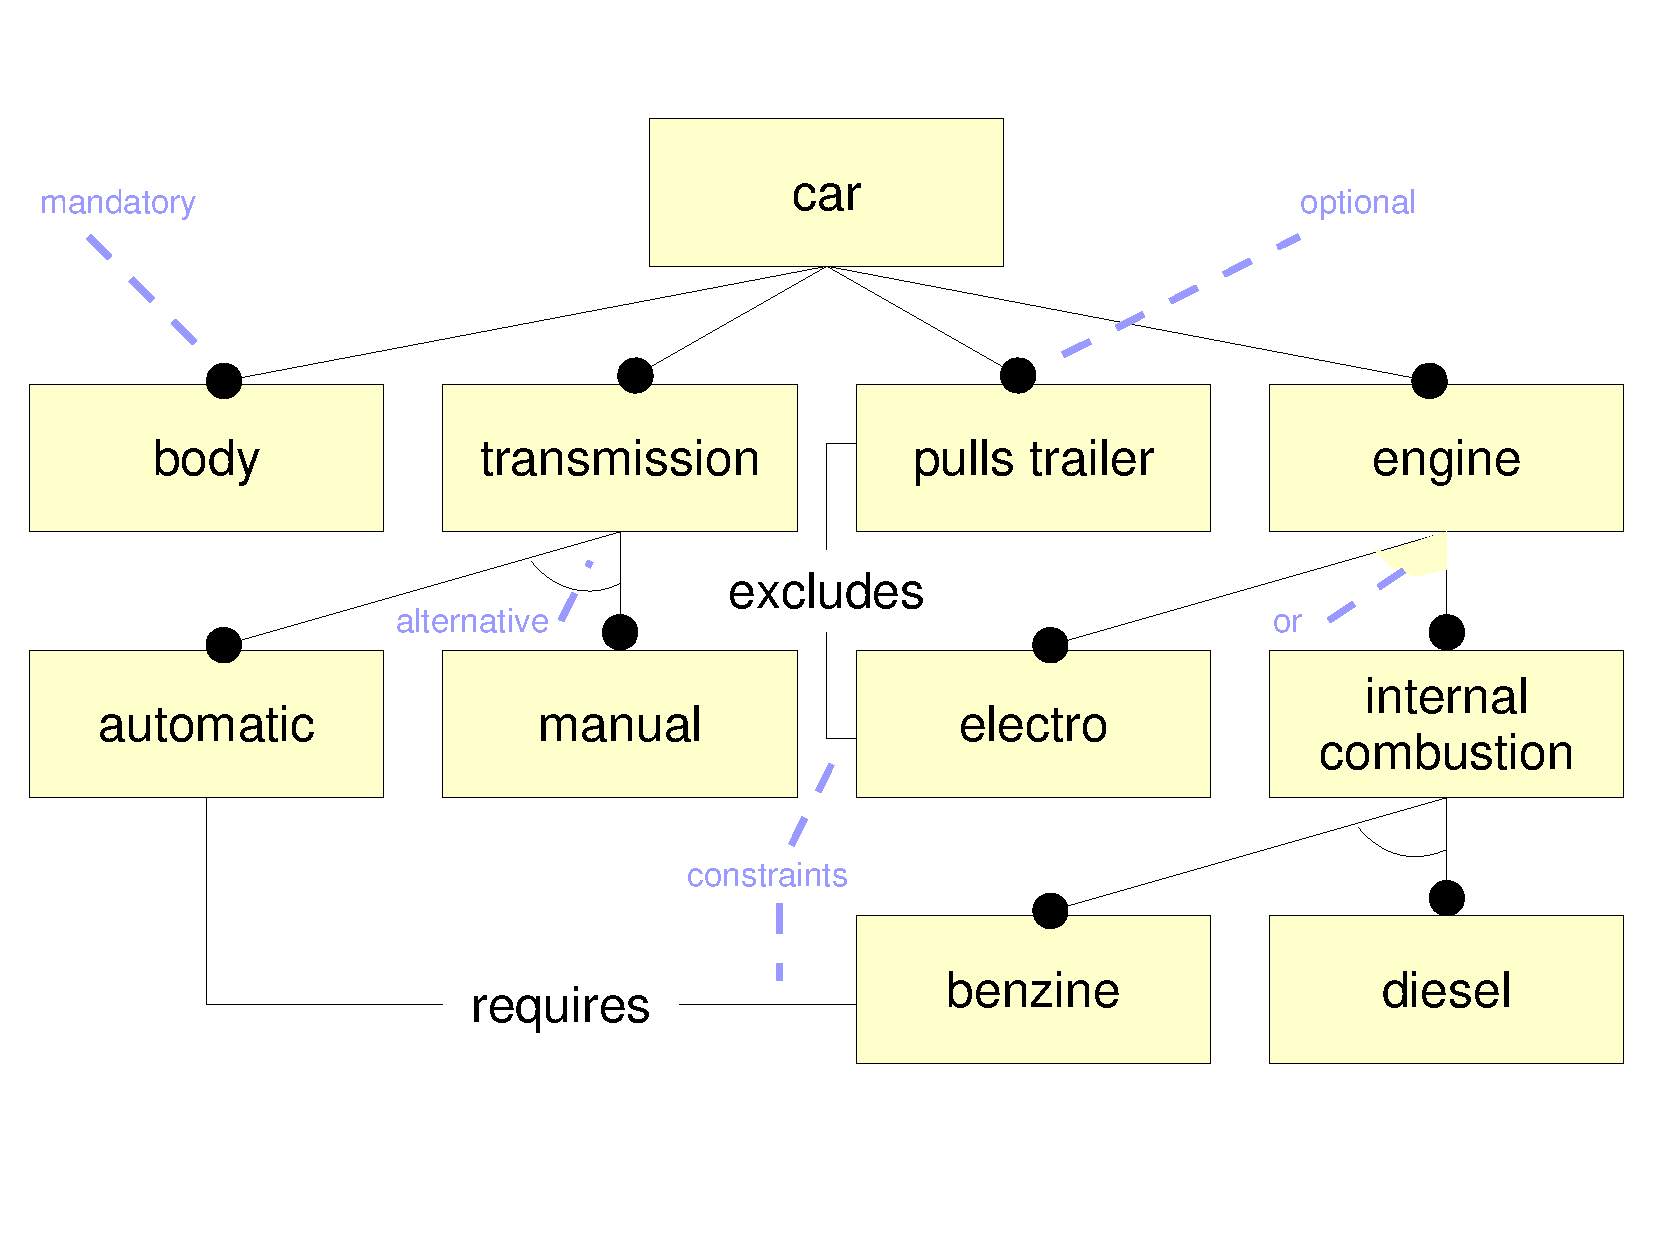
\includegraphics[scale=0.3,angle=-90]{graphic/feature.pdf}
        \caption{Classical Feature Model Diagram of a Car (based on \cite{pashov})}
        \label{feature_figure}
    \end{center}
\end{figure}

In other words, a feature model (figure \ref{feature_figure}) is an additional
form of abstraction within a \emph{Software Engineering Process} (SEP), placed
between analysis- and design models. The properties contained in a feature model
are structured hierarchically. In the \emph{Feature Oriented Domain Analysis}
(FODA) \cite{foda}, a feature model distinguishes three kinds of features:
\emph{Context}, \emph{Representation}, \emph{Operational}. Detlef Streitferdt
\cite{streitferdt200412} defines five feature types:

\begin{enumerate}
    \item \emph{Functional:} used by customer to compose a system
    \item \emph{Interface:} describe required and provided component interfaces
    \item \emph{Parameter:} used to configure functional features
    \item \emph{Structural:} relevant for an automated choice of components
    \item \emph{Conditional:} summarise sub-features to improve readability
\end{enumerate}

Using feature models, the \emph{Traceability} between concrete requirements and
architecture components can be improved. Requirements can better be mapped to
architecture elements, so that also the \emph{Communication} between
stakeholders in the development process can profit. The big abstraction gap
(number \emph{1} in figure \ref{gaps_figure} of section
\ref{abstraction_gaps_heading}) gets split into two smaller (\emph{1a} and
\emph{1b} in figure \ref{gaps_figure}) that do not close the gap conclusively,
but make it easier to cross. The disadvantage of using feature models in a SEP,
however, is that another abstraction gap causing additional effort is created
through them.

The knowledge schema and language introduced in chapters
\ref{knowledge_schema_heading} and \ref{cybernetics_oriented_language_heading}
use a hierarchical structure comparable to the feature model. Their elements,
though, do belong to just one of two possible kinds: \emph{whole-part} model or
\emph{meta property} model. CYBOP knowledge models merge \emph{some} of the
information that would traditionally be found in feature models with that
contained in the design diagrams and might thus be able to eliminate gap 1b.
Non-functional requirements like \emph{Performance}, \emph{Scalability},
\emph{Usability} or \emph{Memory Efficiency} are \emph{not} part of a CYBOP
knowledge model, since they have nothing to do with the actual modelling of
real-world items in form of abstract concepts and belong into a corresponding
analysis- and specification document only.


%
% $RCSfile: generative_programming.tex,v $
%
% Copyright (C) 2002-2008. Christian Heller.
%
% Permission is granted to copy, distribute and/or modify this document
% under the terms of the GNU Free Documentation License, Version 1.1 or
% any later version published by the Free Software Foundation; with no
% Invariant Sections, with no Front-Cover Texts and with no Back-Cover
% Texts. A copy of the license is included in the section entitled
% "GNU Free Documentation License".
%
% http://www.cybop.net
% - Cybernetics Oriented Programming -
%
% http://www.resmedicinae.org
% - Information in Medicine -
%
% Version: $Revision: 1.1 $ $Date: 2008-08-19 20:41:06 $ $Author: christian $
% Authors: Christian Heller <christian.heller@tuxtax.de>
%

\subsection{Generative Programming}
\label{generative_programming_heading}
\index{Generative Programming}
\index{GP}
\index{Aspect Oriented Programming}
\index{AOP}
\index{Generic Programming}
\index{Domain Specific Language}
\index{DSL}
\index{Feature Model}
\index{Generator}
\index{Model Driven Architecture}
\index{MDA}

\emph{Generative Programming} (GP), as proposed by Czarnecki \cite{czarnecki},
is \textit{a comprehensive software development paradigm to achieving high
intentionality, reusability, and adaptability without the need to compromise
the runtime performance and computing resources of the produced software.} It
encompasses techniques of the following, previously described paradigms:

\begin{itemize}
    \item[-] \emph{Aspect Oriented Programming} (AOP) (section
        \ref{aspect_oriented_programming_heading}): used to achieve separation
        of concerns
    \item[-] \emph{Generic Programming} (section \ref{generics_heading}): used
        to parameterise over types
    \item[-] \emph{Domain Specific Language} (DSL) (section
        \ref{domain_specific_language_heading}): used to improve
        intentionality, optimisation and error checking of program code
    \item[-] \emph{Feature Model} (section \ref{feature_model_heading}): used
        as configuration knowledge, to map between problem- and solution space
\end{itemize}

Czarnecki's work contributes to the formal specification and extension of the
\emph{Feature Model}, but does not itself deliver new forms of knowledge
abstraction. GP, however, is mentioned here because of its idea of applying
\emph{Generators} (or generative techniques) producing implementation source
code for a software system from the higher-level specifications defined in the
design phase. Similar techniques are used in the
\emph{Model Driven Architecture} (see next section). GP is a trial to automate
the process of crossing abstraction gap number \emph{2} (with reference to
figure \ref{gaps_figure}), and it is often quite successful. However, the gap
between architecture design models and program source code remains. Chapter
\ref{knowledge_schema_heading} will introduce a \emph{Knowledge Schema} serving
as universal type, so that differing type-based architectures do not have to be
designed anymore.

%
% $RCSfile: model_driven_architecture.tex,v $
%
% Copyright (C) 2002-2008. Christian Heller.
%
% Permission is granted to copy, distribute and/or modify this document
% under the terms of the GNU Free Documentation License, Version 1.1 or
% any later version published by the Free Software Foundation; with no
% Invariant Sections, with no Front-Cover Texts and with no Back-Cover
% Texts. A copy of the license is included in the section entitled
% "GNU Free Documentation License".
%
% http://www.cybop.net
% - Cybernetics Oriented Programming -
%
% http://www.resmedicinae.org
% - Information in Medicine -
%
% Version: $Revision: 1.1 $ $Date: 2008-08-19 20:41:07 $ $Author: christian $
% Authors: Christian Heller <christian.heller@tuxtax.de>
%

\subsection{Model Driven Architecture}
\label{model_driven_architecture_heading}
\index{Model Driven Architecture}
\index{MDA}
\index{Object Management Group}
\index{OMG}
\index{Unified Modeling Language}
\index{UML}
\index{Meta Object Facility}
\index{MOF}
\index{Interface Definition Language}
\index{IDL}
\index{XML Metadata Interchange}
\index{XMI}
\index{Extensible Markup Language}
\index{XML}
\index{Common Warehouse Metamodel}
\index{CWM}
\index{Common Object Request Broker Architecture}
\index{CORBA}
\index{Platform Independent Model}
\index{PIM}
\index{Platform Specific Model}
\index{PSM}
\index{Computer Aided Software Engineering Tool}
\index{CASE Tool}
\index{DE}
\index{DE}
\index{DE}
\index{DE}

The \emph{Model Driven Architecture} (MDA) \cite{mda} (figure \ref{mda_figure}),
an approach to application design and implementation \cite{brown2004} specified
by the \emph{Object Management Group} (OMG), represents a suite of key
standards including:

\begin{itemize}
    \item[-] \emph{Unified Modeling Language} (UML): modelling, visualising and
        documenting the structure and behaviour of systems using graphical
        diagrams
    \item[-] \emph{Meta Object Facility} (MOF): representing and manipulating
        meta models using CORBA and its \emph{Interface Definition Language}
        (IDL); UML can be expressed in terms of MOF, which is done to generate
        XMI
    \item[-] \emph{XML Metadata Interchange} (XMI): interchanging UML
        metamodels and models using an \emph{Extensible Markup Language}
        (XML)-based format
    \item[-] \emph{Common Warehouse Metamodel} (CWM): enabling data mining
        across database boundaries at an enterprise using a complete,
        comprehensive metamodel; does for data modelling what UML does for
        application modelling
    \item[-] \emph{Common Object Request Broker Architecture} (CORBA):
        communicating using a programming language-, operating system- and
        vendor-independent middleware platform
\end{itemize}

\begin{figure}[ht]
    \begin{center}
        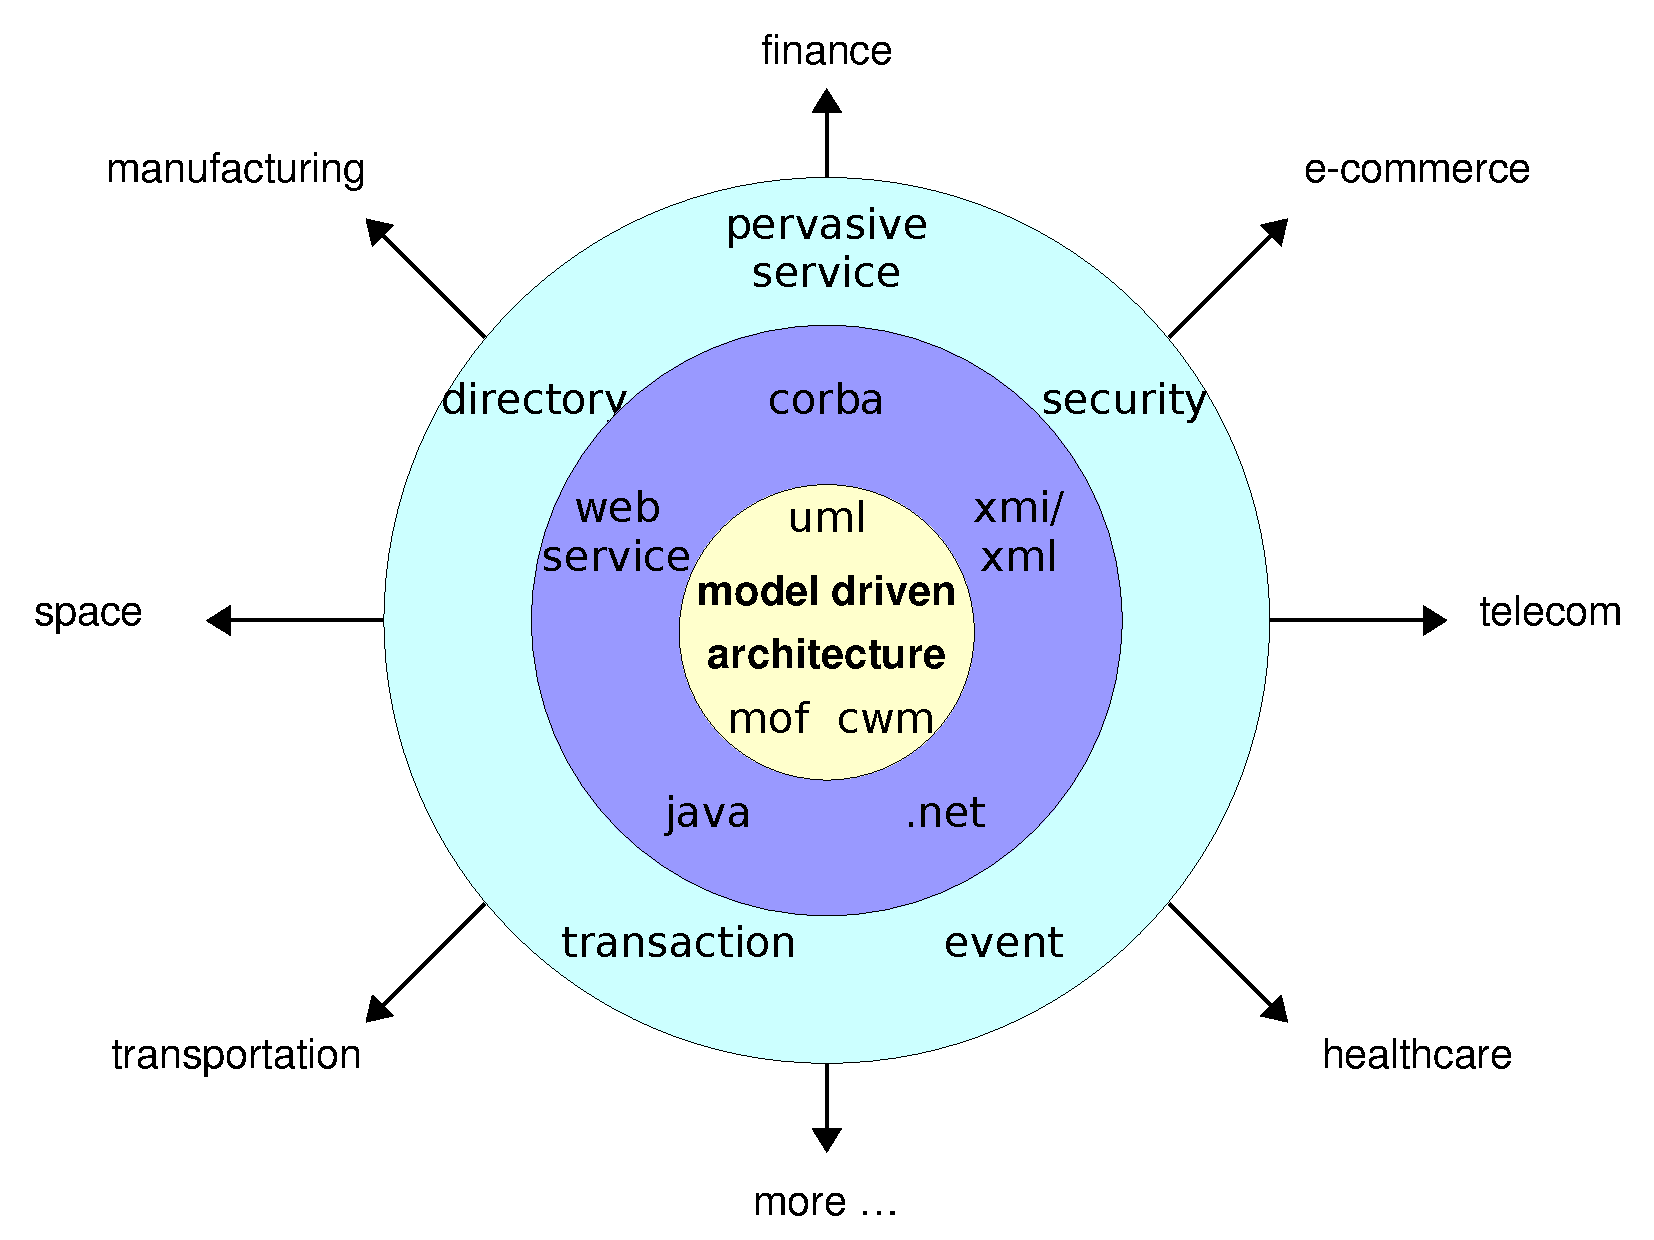
\includegraphics[scale=0.3,angle=-90]{graphic/mda.pdf}
        \caption{Model Driven Architecture \cite{mda}}
        \label{mda_figure}
    \end{center}
\end{figure}

Brown \cite{brown2004} writes: \textit{MDA encourages efficient use of system
models in the software development process, and it supports reuse of best
practices when creating families of systems.} In the OMG's own words, MDA is a:
\textit{way to organise and manage enterprise architectures supported by
automated tools and services for both defining the models and facilitating
transformations between different model types.} It aims at providing an:
\textit{open, vendor-neutral approach to the challenge of business- and
technology change}.

While traditional approaches like \emph{System Family} or
\emph{Tools \& Materials} (section \ref{tool_and_material_heading}) merely
distinguish between \emph{Domain} and \emph{Application}, the conceptual
framework provided by the MDA takes another step in separating abstract
knowledge: It treats \emph{Platform Independent Models} (PIM), that is
business- or application logic, different than the underlying
\emph{Platform Specific Models} (PSM), that is implementation technology. The
translation between the two kinds of models is normally performed using
automated tools for code generation (section \ref{generative_programming_heading}).

The MDA claims to overcome the limitations of implementation
technology-dependent \emph{Computer Aided Software Engineering} (CASE) tools
via standardised mappings and meta architectures \`a la MOF \cite{frankel}.
After Martin Fowler \cite{fowlerdsl}, one argument used in favor of MDA were
that it makes it possible to use \emph{Domain Specific Languages} (DSL)
(section \ref{domain_specific_language_heading}). However, he doubts a success
of the MDA. And indeed, although some MDA standards like the UML are very
sophisticated and widely used, it is still unclear whether the MDA, due to its
complexity, will be able to infiltrate daily software business.

But the idea of separating \emph{Application Knowledge} (PIM) from its
hardware-close \emph{Control and Processing} (PSM) clearly brings a new quality
into software development and is important for later investigations in this
work (chapter \ref{statics_and_dynamics_heading}).

%
% $RCSfile: model_and_code.tex,v $
%
% Copyright (C) 2002-2008. Christian Heller.
%
% Permission is granted to copy, distribute and/or modify this document
% under the terms of the GNU Free Documentation License, Version 1.1 or
% any later version published by the Free Software Foundation; with no
% Invariant Sections, with no Front-Cover Texts and with no Back-Cover
% Texts. A copy of the license is included in the section entitled
% "GNU Free Documentation License".
%
% http://www.cybop.net
% - Cybernetics Oriented Programming -
%
% http://www.resmedicinae.org
% - Information in Medicine -
%
% Version: $Revision: 1.1 $ $Date: 2008-08-19 20:41:07 $ $Author: christian $
% Authors: Christian Heller <christian.heller@tuxtax.de>
%

\subsection{Model and Code}
\label{model_and_code_heading}
\index{Model-Code Synchronisation}
\index{Code Only Approach}
\index{Code Visualisation Approach}
\index{Roundtrip Engineering Approach}
\index{Model Centric Approach}
\index{Model Only Approach}
\index{Model Driven Architecture}
\index{MDA}
\index{Design Phase}
\index{Implementation Phase}
\index{Software Engineering Process}
\index{SEP}

The knowledge abstraction- and implementation techniques considered in the
previous sections belong to the current state-of-the-art in software design and
-modelling, with focus on \emph{Domain Engineering} (DE). Despite some
exceptions like the \emph{Feature Model} (section \ref{feature_model_heading}),
which supports the mapping between abstractions of the analysis- and design
phase, most described techniques deal with bridging the gap between design
models and source code.

\begin{figure}[ht]
    \begin{center}
        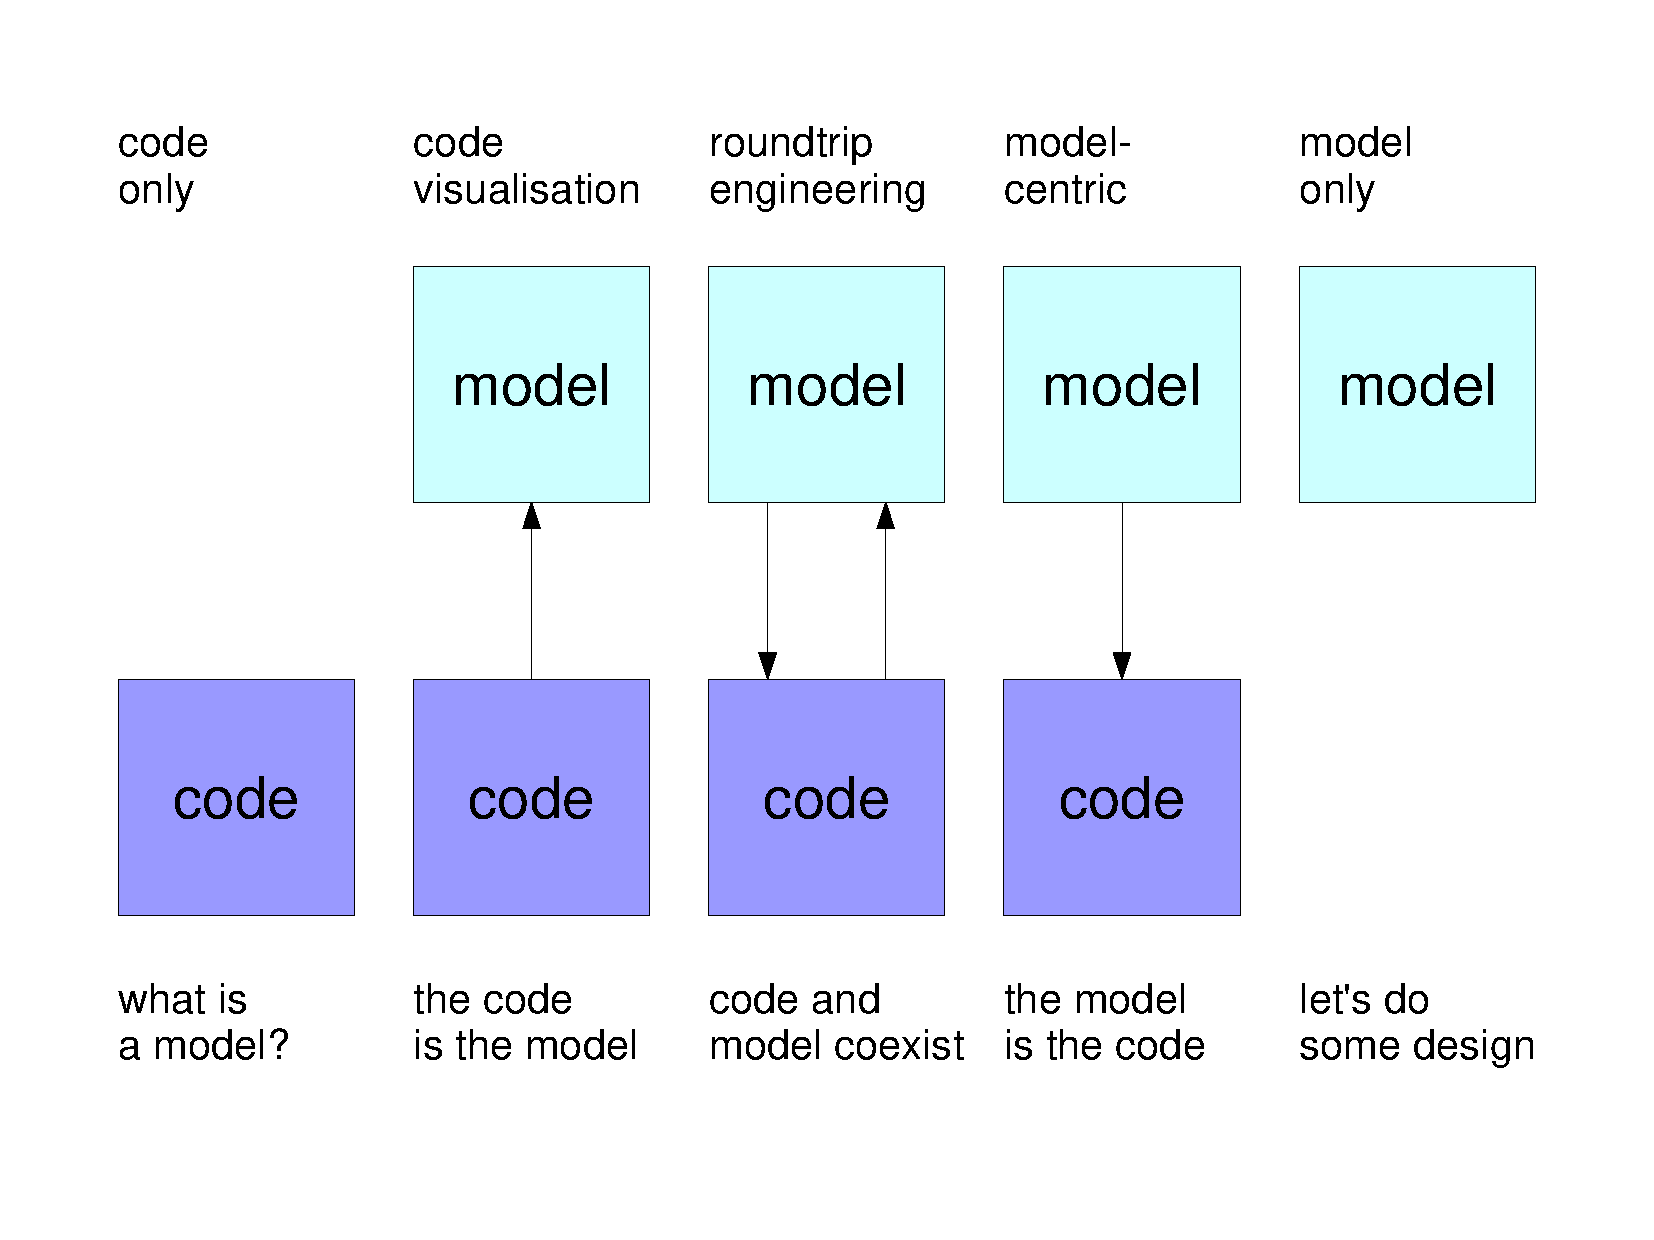
\includegraphics[scale=0.3,angle=-90]{graphic/modelcode.pdf}
        \caption{Model-Code Synchronisation \cite[diagram by John Daniels]{brown2004}}
        \label{modelcode_figure}
    \end{center}
\end{figure}

Alan Brown writes \cite{brown2004}: \textit{One useful way to characterise current
practice is to look at the different ways in which the models are synchronized
with the source code they help describe.} Figure \ref{modelcode_figure} shows
the spectrum of modelling approaches in use today. The different categories
\cite{brown2004} are:

%
% $RCSfile: code_only.tex,v $
%
% Copyright (C) 2002-2008. Christian Heller.
%
% Permission is granted to copy, distribute and/or modify this document
% under the terms of the GNU Free Documentation License, Version 1.1 or
% any later version published by the Free Software Foundation; with no
% Invariant Sections, with no Front-Cover Texts and with no Back-Cover
% Texts. A copy of the license is included in the section entitled
% "GNU Free Documentation License".
%
% http://www.cybop.net
% - Cybernetics Oriented Programming -
%
% http://www.resmedicinae.org
% - Information in Medicine -
%
% Version: $Revision: 1.1 $ $Date: 2008-08-19 20:41:05 $ $Author: christian $
% Authors: Christian Heller <christian.heller@tuxtax.de>
%

\subsubsection{Code Only}
\label{code_only_heading}

\begin{itemize}
    \item[-] almost entire reliance on the code
    \item[-] informal and intuitive modelling of architectural designs
    \item[-] models living on whiteboards, in presentations or the developers' heads
    \item[-] possible use of an \emph{Integrated Development Environment} (IDE)
\end{itemize}

%
% $RCSfile: code_visualisation.tex,v $
%
% Copyright (C) 2002-2008. Christian Heller.
%
% Permission is granted to copy, distribute and/or modify this document
% under the terms of the GNU Free Documentation License, Version 1.1 or
% any later version published by the Free Software Foundation; with no
% Invariant Sections, with no Front-Cover Texts and with no Back-Cover
% Texts. A copy of the license is included in the section entitled
% "GNU Free Documentation License".
%
% http://www.cybop.net
% - Cybernetics Oriented Programming -
%
% http://www.resmedicinae.org
% - Information in Medicine -
%
% Version: $Revision: 1.1 $ $Date: 2008-08-19 20:41:05 $ $Author: christian $
% Authors: Christian Heller <christian.heller@tuxtax.de>
%

\subsubsection{Code Visualisation}
\label{code_visualisation_heading}

\begin{itemize}
    \item[-] alternative modelling using a graphical notation
    \item[-] diagrams aid the understanding of the code's structure or behavior
    \item[-] visual renderings become a direct representation of the code
    \item[-] simultaneous display of code view and model view using
        \emph{Computer Aided Software Engineering} (CASE) tools
\end{itemize}

%
% $RCSfile: roundtrip_engineering.tex,v $
%
% Copyright (C) 2002-2008. Christian Heller.
%
% Permission is granted to copy, distribute and/or modify this document
% under the terms of the GNU Free Documentation License, Version 1.1 or
% any later version published by the Free Software Foundation; with no
% Invariant Sections, with no Front-Cover Texts and with no Back-Cover
% Texts. A copy of the license is included in the section entitled
% "GNU Free Documentation License".
%
% http://www.cybop.net
% - Cybernetics Oriented Programming -
%
% http://www.resmedicinae.org
% - Information in Medicine -
%
% Version: $Revision: 1.1 $ $Date: 2008-08-19 20:41:08 $ $Author: christian $
% Authors: Christian Heller <christian.heller@tuxtax.de>
%

\subsubsection{Roundtrip Engineering}
\label{roundtrip_engineering_heading}

\begin{itemize}
    \item[-] bidirectional exchange between abstract design model and
        implementation code
    \item[-] manual model-to-code transformation, and vice-versa
    \item[-] frequent iterations as errors are detected
    \item[-] considerable discipline necessary to keep models synchronized
    \item[-] automated recognition of generated versus user-defined code by
        \emph{Roundtrip Engineering} (RTE) tools (for example by placing markers
        in the code)
\end{itemize}

%
% $RCSfile: model_centric.tex,v $
%
% Copyright (C) 2002-2008. Christian Heller.
%
% Permission is granted to copy, distribute and/or modify this document
% under the terms of the GNU Free Documentation License, Version 1.1 or
% any later version published by the Free Software Foundation; with no
% Invariant Sections, with no Front-Cover Texts and with no Back-Cover
% Texts. A copy of the license is included in the section entitled
% "GNU Free Documentation License".
%
% http://www.cybop.net
% - Cybernetics Oriented Programming -
%
% http://www.resmedicinae.org
% - Information in Medicine -
%
% Version: $Revision: 1.1 $ $Date: 2008-08-19 20:41:07 $ $Author: christian $
% Authors: Christian Heller <christian.heller@tuxtax.de>
%

\subsubsection{Model Centric}
\label{model_centric_heading}

\begin{itemize}
    \item[-] sufficiently detailed system models enable the generation of full
        system implementations
    \item[-] models include representations of persistent- and non-persistent
        data, business logic, presentation elements and more
    \item[-] interfaces to legacy systems and various services
    \item[-] specialized tools generate particular (constrained) styles of
        applications, in an automated process
\end{itemize}

%
% $RCSfile: model_only.tex,v $
%
% Copyright (C) 2002-2008. Christian Heller.
%
% Permission is granted to copy, distribute and/or modify this document
% under the terms of the GNU Free Documentation License, Version 1.1 or
% any later version published by the Free Software Foundation; with no
% Invariant Sections, with no Front-Cover Texts and with no Back-Cover
% Texts. A copy of the license is included in the section entitled
% "GNU Free Documentation License".
%
% http://www.cybop.net
% - Cybernetics Oriented Programming -
%
% http://www.resmedicinae.org
% - Information in Medicine -
%
% Version: $Revision: 1.1 $ $Date: 2008-08-19 20:41:07 $ $Author: christian $
% Authors: Christian Heller <christian.heller@tuxtax.de>
%

\subsubsection{Model Only}
\label{model_only_heading}

\begin{itemize}
    \item[-] models aid the understanding of a business domain, or the analysing
        of a proposed architecture
    \item[-] models used as basis for discussion, communication and analysis
        among project teams within- or across organisations
    \item[-] establishment of a shared vocabulary and set of concepts among
        disparate teams
    \item[-] model-disconnected (outsourced) implementation of systems
\end{itemize}


Considering the developments of the last decades but especially recent years,
the modelling trend clearly goes \emph{left-to-right}, with respect to figure
\ref{modelcode_figure}, that is from \emph{Code only-} to more \emph{Model-centric}
approaches. The emerge of the \emph{Model Driven Architecture} (MDA) (section
\ref{model_driven_architecture_heading}) is one sign therefore. Yet although
these efforts certainly contribute to easier and faster development, less
inter-dependencies within systems, better documentation and clearity of source
code, improved maintenance and more -- the gap between \emph{Design-} and
\emph{Implementation} phase, within a \emph{Software Engineering Process} (SEP)
(chapter \ref{software_engineering_process_heading}), remains. By introducing a
new knowledge schema (chapter \ref{knowledge_schema_heading}), this work wants
to conclusively close gap number \emph{2} (with respect to figure
\ref{gaps_figure} of section \ref{abstraction_gaps_heading}) and provide a
model-only approach.

